%% ma: L12-B02-0016
%% lop: 12
%% chuong: 1
%% bai: 2
%% dang: 12.2.11
%% loai: TN4
%% muc: TH
%% dap_an: "D"
%% nguon: "Ảnh giáo viên gửi 05/11/2026 (M11): Kiểm tra giữa HK1 Toán 12 (2026-2027), THPT Hồ Thị Bi (TP.HCM), mã đề 1133, Phần I Câu 4"
%% kien_thuc: "Bài 2 (giá trị lớn nhất, nhỏ nhất của hàm số trên khoảng); Bài 1 (xét dấu đạo hàm, đơn điệu); Bài 3 (giới hạn tại vô cực và giới hạn một phía)"
%% trang_thai: cho-duyet
%% ly_do: "Dạng mới 12.2.11 đang đề xuất, chờ giáo viên duyệt"
%% ghi_chu: "Đề gốc không kèm đáp án; đã giải độc lập."
\begin{ex}
Cho hàm số $y=f(x)$ có đạo hàm $f'(x)$ xác định và liên tục trên khoảng $(-2;+\infty)$; $\displaystyle\lim_{x\to(-2)^+}f(x)=-\infty$, $\displaystyle\lim_{x\to+\infty}f(x)=10$, $f(-1)=5$ và có bảng xét dấu đạo hàm như sau:
\begin{center}
\begin{tikzpicture}
  \tkzTabInit[lgt=1.5,espcl=2.4]{$x$/.8,$f'(x)$/.8}{$-2$,$-1$,$2$,$+\infty$}
  \tkzTabLine{,+,0,-,0,+,}
\end{tikzpicture}
\end{center}
Mệnh đề nào dưới đây đúng?
\choice{$\max\limits_{(-2;+\infty)}f(x)=f(-1)$}{$\max\limits_{(-2;+\infty)}f(x)=10$}{$\min\limits_{(-2;+\infty)}f(x)=f(2)$}{\True Hàm số không có giá trị lớn nhất trên khoảng $(-2;+\infty)$}
\loigiai{Hàm số đồng biến trên $(-2;-1)$ và $(2;+\infty)$, nghịch biến trên $(-1;2)$.
Trên $(2;+\infty)$ hàm số tăng và tiến tới $10$ khi $x\to+\infty$ nên $f(x)<10$ với mọi $x>2$ và $f(x)$ có thể lớn hơn $f(-1)=5$ tùy ý gần $10$; hàm số không đạt giá trị $10$. Vậy không có giá trị lớn nhất (A, B sai).
Vì $\lim\limits_{x\to(-2)^+}f(x)=-\infty$ nên hàm số không có giá trị nhỏ nhất (C sai).}
\end{ex}
